\setcounter{exercisegroup}{2}
\refstepcounter{exercisegroup}
\section*{Exercises on \S\arabic{exercisegroup}}
\phantomsection
\addcontentsline{toc}{section}{Exercises on \protect\S\arabic{exercisegroup}}

\begin{enumerate}
\def\labelenumi{\arabic{enumi})}
\tightlist
\item
  Let I be an arbitrary interval in R, let A be a set, and g a finite real function defined on \(I \times A\) such that for every \(\alpha \in A\) the map \(t \mapsto g(t, \alpha)\) is decreasing and \(\geqslant 0\) on I; suppose further that there is a number M independent of \(\alpha\) such that \(g(t, \alpha) \leqslant M\) on \(I \times A\) .
\end{enumerate}

\begin{enumerate}
\def\labelenumi{\alph{enumi})}
\item
  Show that if \(\mathbf{f}\) is a regulated function on I such that the integral \(\int_{\mathrm{I}} \mathbf{f}(t) dt\) converges, then the integral \(\int_{\mathrm{I}} \mathbf{f}(t) g(t, \alpha) dt\) is uniformly convergent for \(\alpha \in \mathrm{A}\) (use the second mean value theorem; cf.~II, p.~82, exerc. 16).
\item
  Suppose that I = {[}a, +∞{]} and also that \(g(t, \alpha)\) tends uniformly to 0 (for \(\alpha \in A\) ) when t tends to +∞. Show that if f is a regulated function on I and if there is a number k \textgreater{} 0 such that \(\left\|\int_{J} \mathbf{f}(t) dt\right\| \leqslant k\) for every compact interval J contained in I, then the integral \(\int_{I} \mathbf{f}(t) g(t, \alpha) dt\) is uniformly convergent for \(\alpha \in A\) (same method).
\item
  Suppose that \(I = [a, +\infty[\) with a \textgreater{} 0, \(A = [0, +\infty[,\) and \(g(t, \alpha) = \varphi(\alpha t)\) , where \(\varphi\) is a convex decreasing function and \(\geqslant 0\) on A, tending to 0 as x tends to \(+\infty\) and such that \(\varphi(0) = 1\) . Suppose further that \(f = h''\) , where h is a twice differentiable function on \([a, +\infty[,\) and, together with \(h'\) , is bounded on this interval. The integral \(\int_{a}^{+\infty} f(t) \varphi(\alpha t) dt\) is then convergent for \(\alpha > 0\) ; show that when \(\alpha\) tends to 0, it tends to \(-\mathbf{h}'(a)\) (integrate by parts and use the second mean value theorem).
\end{enumerate}

* \(d\) ) Take \(\varphi (x) = e^{-cx}\) , where \(c > 0\) , take \(a = 1\) , and for \(f\) take the complex function \(t\mapsto e^{i\log t} / t\) , which is the derivative of a bounded function on I; show that for a suitable choice of \(c\) the integral \(\int_{1}^{+\infty}e^{-\alpha ct}\frac{e^{i\log t}}{t} dt\) , which is absolutely convergent for \(\alpha >0\) , does not tend to any limit when \(\alpha\) tends to 0 (after integrating by parts, make the change of variables \(\alpha t = u\) ; use Laplace transform theory to see that \(\int_0^{+\infty}e^{-cu + i\log u}du\) does not vanish for certain \(c > 0\) .)*

\begin{enumerate}
\def\labelenumi{\arabic{enumi})}
\setcounter{enumi}{1}
\tightlist
\item
  Let \(f\) and \(g\) be two real regulated functions on a compact interval \([a, b]\) , such that \(f\) is decreasing on \([a, b]\) , and \(0 \leqslant g(t) \leqslant 1\) . If one puts \(\lambda = \int_{a}^{b} g(t) dt\) , show that one has
\end{enumerate}

\[
\int_ {b - \lambda} ^ {b} f (t) d t <   \int_ {a} ^ {b} f (t) g (t) d t <   \int_ {a} ^ {a + \lambda} f (t) d t
\]

except when f is constant, or g is equal to 0 (resp. 1) at all the points where it is continuous (in which case all three terms are equal). (Vary one of the limits of integration in the integral \(\int_{x}^{y} f(t)g(t)dt\) .)

\begin{enumerate}
\def\labelenumi{\arabic{enumi})}
\setcounter{enumi}{2}
\tightlist
\item
  Let \(f(x, \alpha) = 1 / \sqrt{1 - 2\alpha x + \alpha^2}\) for \(-1 < x < +1\) and \(\alpha \in \mathbf{R}\) ; show that the function \(g(\alpha) = \int_{-1}^{+1} dx / \sqrt{1 - 2\alpha x + \alpha^2}\) is continuous on \(\mathbf{R}\) , but has no derivative at \(\alpha = 1\) and \(\alpha = -1\) ; show that \(f_{\alpha}'(x, \alpha)\) exists for all \(\alpha \in \mathbf{R}\) and for \(x \in I = ] - 1, +1[\) , and is continuous on \(I \times R\) , and that the integral \(\int_{-1}^{+1} f_{\alpha}'(x, \alpha) dx\) exists for all \(\alpha \in R\) , but verify that this integral is not uniformly convergent on a neighbourhood of the point \(\alpha = 1\) or of the point \(\alpha = -1\) .
\end{enumerate}

¶ 4) Let I be an interval of \(\mathbf{R}\) , A a neighbourhood of a point \(\alpha_0\) in the field \(\mathbf{R}\) (resp. the field \(\mathbf{C}\) ), and \(\mathbf{f}\) a continuous map of \(\mathrm{I} \times \mathrm{A}\) into a complete normed space \(\mathrm{E}\) over \(\mathbf{R}\) , such that \(\mathbf{f}_{\alpha}'(x, \alpha)\) exists and is continuous on \(\mathrm{I} \times \mathrm{A}\) . Let \(a(\alpha)\) , \(b(\alpha)\) be two continuous functions defined on A, with values in I, such that one has identically \(\mathbf{f}(a(\alpha), \alpha) = \mathbf{f}(b(\alpha), \alpha) = 0\) on A. Show that the function \(\mathbf{g}(\alpha) = \int_{a(\alpha)}^{b(\alpha)} \mathbf{f}(t, \alpha) dt\) admits a derivative equal to \(\int_{a(\alpha_0)}^{b(\alpha_0)} \mathbf{f}_{\alpha}'(t, \alpha_0) dt\) at the point \(\alpha_0\) , even if \(a\) and \(b\) are not differentiable at the point \(\alpha_0\) (let M be the supremum of \(\left\| \mathbf{f}_{\alpha}'(x, \alpha) \right\|\) on a compact neighbourhood of \((b(\alpha_0), \alpha_0)\) ; note, applying Bolzano's theorem to \(b(\alpha)\) , that for every \(x\) belonging to the interval with endpoints \(b(\alpha_0)\) and \(b(\alpha)\) , one has, for \(\alpha\) sufficiently close to \(\alpha_0\) , that \(\| \mathbf{f}(x, \alpha) \| \leqslant M |\alpha - \alpha_0|\) ).

\begin{enumerate}
\def\labelenumi{\arabic{enumi})}
\setcounter{enumi}{4}
\tightlist
\item
  Let \(\mathbf{f}\) be a continuous vector function on a compact interval \(I = [0, a]\) . Show that if, at the point \(\alpha_0 \in I\) , there is an \(\varepsilon > 0\) such that \((\mathbf{f}(x) - \mathbf{f}(\alpha_0)) / |x - \alpha_0|^{1/2 + \varepsilon}\) remains bounded as \(x\) tends to \(\alpha_0\) , then the function \(\mathbf{g}(\alpha) = \int_0^\alpha \mathbf{f}(x) dx / \sqrt{\alpha - x}\) admits a derivative equal to
\end{enumerate}

\[
\frac {1}{\sqrt {\alpha_ {0}}} \mathbf {f} (\alpha_ {0}) - \frac {1}{2} \int_ {0} ^ {\alpha_ {0}} \frac {\mathbf {f} (x) - \mathbf {f} (\alpha_ {0})}{(\alpha_ {0} - x) ^ {3 / 2}} d x
\]

at the point \(\alpha_0\) for \(\alpha_0 > 0\) , and to 0 for \(\alpha = 0\) .

When \(\mathbf{f}\) is the real function \(\sqrt{\alpha_0 - x}\) , show that the function \(\mathbf{g}\) has an infinite derivative at the point \(\alpha_0\) .

¶ 6) Let \(\mathrm{I} = [a, b]\) , \(\mathrm{A} = [c, d]\) be two compact intervals on \(\mathbf{R}\) ; let \(\mathbf{f}\) be a function defined on \(\mathrm{I} \times \mathrm{A}\) , with values in a complete normed space \(\mathrm{E}\) over \(\mathbf{R}\) , such that for all \(\alpha \in \mathrm{A}\) , the map \(t \mapsto \mathbf{f}(t, \alpha)\) is regulated on \(\mathrm{I}\) , that \(\mathbf{f}\) is bounded on \(\mathrm{I} \times \mathrm{A}\) , and that the set \(\mathrm{D}\) of points of discontinuity of \(\mathbf{f}\) in \(\mathrm{I} \times \mathrm{A}\) is met in a finite number of points by each line \(x = x_0\) and each line \(\alpha = \alpha_0\) ( \(x_0 \in \mathrm{I}\) , \(\alpha_0 \in \mathrm{A}\) ).

\begin{enumerate}
\def\labelenumi{\alph{enumi})}
\item
  Show that the function \(\mathbf{g}(\alpha) = \int_{a}^{b} \mathbf{f}(t, \alpha) dt\) is continuous on A (given \(\alpha_0 \in \mathrm{A}\) and \(\varepsilon > 0\) , show that there is a neighbourhood V of \(\alpha_0\) and a finite number of intervals \(J_k\) contained in I with the sum of their lengths \(\leqslant \varepsilon\) , such that, if J denotes the complement in I of \(\bigcup_{k} J_k\) , then \(\mathbf{f}\) is continuous on \(\mathrm{J} \times \mathrm{V}\) ).
\item
  Show that the formula for interchanging the order of integration (II, p.~77, formula (15)) is still valid (same method as in a)).
\end{enumerate}

\begin{enumerate}
\def\labelenumi{\arabic{enumi})}
\setcounter{enumi}{6}
\tightlist
\item
  Let \(f\) be a real function defined and having a continuous derivative on the interval \(]0, +\infty[\) , and such that
\end{enumerate}

\[
\lim _ {x \to 0} f (x) = \lim _ {x \to + \infty} f (x) = 0.
\]

The integral \(\int_0^{+\infty}f'(\alpha t)dt\) is defined and continuous on every bounded interval \(]0,a]\) ; show that the integral \(\int_0^{+\infty}dt\int_0^a f'(\alpha t)d\alpha\) may either not exist or may be different from

\[
\int_ {0} ^ {a} d \alpha \int_ {0} ^ {+ \infty} f ^ {\prime} (\alpha t) d t.
\]

¶ 8) Let \(I\) and \(J\) be two arbitrary intervals in \(\mathbf{R}\) , and \(\mathbf{f}\) a function defined and continuous on \(I \times J\) , with values in a complete normed space \(E\) over \(\mathbf{R}\) . Suppose that:

\(1^{\circ}\) the integral \(\int_{\mathrm{I}}\mathbf{f}(x,y)dx\) is uniformly convergent when \(y\) runs through an arbitrary compact interval contained in J;

\(2^{\circ}\) the integral \(\int_{\mathrm{J}}\mathbf{f}(x,y)dy\) is uniformly convergent when \(x\) runs through an arbitrary compact interval contained in I;

\(3^{\circ}\) if, for every compact interval \(\mathrm{H}\) contained in I, one puts \(\mathbf{u}_{\mathrm{H}}(y) = \int_{\mathrm{H}} \mathbf{f}(x, y) dx\) , the integral \(\int_{\mathrm{J}} \mathbf{u}_{\mathrm{H}}(y) dy\) is uniformly convergent for \(\mathrm{H} \in \mathfrak{K}(\mathrm{I})\) (the right directed ordered set of compact intervals contained in I).

Under these conditions, show that the integrals \(\int_{\mathrm{I}} dx \int_{\mathrm{J}} \mathbf{f}(x, y) dy\) and \(\int_{\mathrm{J}} dy \int_{\mathrm{I}} \mathbf{f}(x, y) dx\) exist and are equal.

* 9) Deduce from exerc. 8 that the integrals

\[
\int_ {0} ^ {\infty} d x \int_ {0} ^ {\infty} e ^ {- y x ^ {2}} \sin y d y \quad \text { and } \quad \int_ {0} ^ {\infty} d y \int_ {0} ^ {\infty} e ^ {- y x ^ {2}} \sin y d x
\]

exist and are equal.*

\begin{enumerate}
\def\labelenumi{\arabic{enumi})}
\setcounter{enumi}{9}
\tightlist
\item
  \begin{enumerate}
  \def\labelenumii{\alph{enumii})}
  \tightlist
  \item
    If \(h, u, v'\) are primitives of real regulated functions on an open interval \(]a, b[\) of \(\mathbf{R}\) , if \(v\) is a primitive of \(v'\) , and if \(v(x) > 0\) on this interval, then one has the Redheffer identity
  \end{enumerate}
\end{enumerate}

\[
h u ^ {\prime 2} = - h \mathrm{D} \left(\frac {h v ^ {\prime}}{v}\right) + h v ^ {2} \left(\mathrm{D} \left(\frac {u}{v}\right)\right) ^ {2} + \mathrm{D} \left(\frac {u ^ {2} h v ^ {\prime}}{v}\right)
\]

at those points of {]}a, b{[} where the derivatives are defined.

* b) Let \(v\) , \(w\) be two functions \(> 0\) on \(]a\) , \(b[\) , which are primitives of regulated functions \(v' > 0\) , \(w' \leqslant 0\) . Deduce from \(a)\) that for every function \(u\) which is a primitive of a regulated function \(u'\) on \(]a\) , \(b[\) and such that \(\liminf_{x \to a, x > a} u(x) = 0\) , the hypothesis that the integral \(\int_{a}^{b} \frac{w(x)}{v'(x)} u'^2(x) dx\) is convergent implies that the integral \(\int_{a}^{b} \frac{w'(x)}{v(x)} u^2(x) dx\) is convergent and that

\[
\limsup _ {x \to b, x <   b} u ^ {2} (x) w (x) / v (x)
\]

is finite, and also the inequality

\[
\int_ {a} ^ {b} \frac {w (x)}{v ^ {\prime} (x)} u ^ {\prime 2} (x) d x \geqslant - \int_ {a} ^ {b} \frac {w ^ {\prime} (x)}{v (x)} u ^ {2} (x) d x + \operatorname * {l i m s u p} _ {x \to b, x <   b} \frac {u ^ {2} (x) w (x)}{v (x)}.\tag{*}
\]

(Putting \(h = w / v'\) , first observe that \(\int_{c}^{x} dt / h(t) \leqslant v(x) / w(x)\) for \(a < c < x < b\) and remark that by the Cauchy-Schwarz inequality

\[
(u (x) - u (c)) ^ {2} \leqslant \left(\int_ {c} ^ {x} h (t) u ^ {\prime 2} (t) d t\right) \left(\int_ {c} ^ {x} \frac {d t}{h (t)}\right),\tag{**}
\]

to deduce that

\[
\liminf _ {x \to a, x > a} u ^ {2} (x) w (x) / v (x) = 0,
\]

and then integrate the Redheffer identity.)

\begin{enumerate}
\def\labelenumi{\alph{enumi})}
\setcounter{enumi}{2}
\tightlist
\item
  Deduce from (*) that if u is the primitive of a regulated function on {]}0, 1{]}, if
\end{enumerate}

\[
\liminf _ {x \to 0, x > 0} u (x) = 0
\]

and if the integral \(\int_0^1 u'^2 (t)dt\) converges, then so does \(\int_0^1 (u(t) / t)^2 dt\) and for all \(\alpha > 0\) one has the inequality

\[
\int_ {0} ^ {1} u ^ {\prime 2} (t) d t \geqslant \alpha (1 - \alpha) \int_ {0} ^ {1} \left(\frac {u (t)}{t}\right) ^ {2} d t + \alpha u ^ {2} (1).
\]

\begin{enumerate}
\def\labelenumi{\alph{enumi})}
\setcounter{enumi}{3}
\tightlist
\item
  Let \(\alpha\) be a number \textgreater0, let K be a function \textgreater0, differentiable and decreasing on \(]0, +\infty[\) and such that \(\lim_{x \to +\infty} K(x) = 0\) . If u is the primitive of a regulated function on \(]0, +\infty[,\) such that \(\liminf_{x \to 0, x > 0} u(x) = 0\) , and if the integral \(\int_{0}^{+\infty} x^{1-\alpha} K(x) u'^{2}(x) dx\) converges, then the function \(x^{-\alpha} K(x) u^{2}(x)\) tends to 0 as x tends to 0 or to \(+\infty\) , the integral
\end{enumerate}

\[
\int_ {0} ^ {+ \infty} x ^ {- \alpha} \mathrm{K} ^ {\prime} (x) u ^ {2} (x) d x
\]

converges, and one has

\[
\int_ {0} ^ {+ \infty} x ^ {1 - \alpha} \mathrm{K} (x) u ^ {\prime 2} (x) d x \geqslant - \alpha \int_ {0} ^ {+ \infty} x ^ {- \alpha} \mathrm{K} ^ {\prime} (x) u ^ {2} (x) d x
\]

(take \(v(x) = x^{\alpha}\) , \(h(x) = x^{1 - \alpha}\mathrm{K}(x)\) in the Redheffer identity).

In particular, for \(\alpha = \frac{1}{2}\) and \(\mathrm{K}(x) = x^{-1 / 2}\) , one has

\[
4 \int_ {0} ^ {+ \infty} u ^ {\prime 2} (x) d x \geqslant \int_ {0} ^ {+ \infty} \left(\frac {u (x)}{x}\right) ^ {2} d x
\]

(Hardy-Littlewood inequality).

\begin{enumerate}
\def\labelenumi{\alph{enumi})}
\setcounter{enumi}{4}
\tightlist
\item
  Let \(\alpha \geqslant -1\) , let \(K\) be a function \(\geqslant 0\) , differentiable and increasing on \([0, +\infty[\) . Suppose that the integrals
\end{enumerate}

\[
\int_ {0} ^ {+ \infty} x ^ {- \alpha} \mathrm{K} (x) u ^ {\prime 2} (x) d x \quad \text { and } \quad \int_ {0} ^ {+ \infty} x ^ {\alpha} \mathrm{K} (x) u ^ {2} (x) d x
\]

converge. Then \(\mathrm{K}(x)u^{2}(x)\) tends to 0 as x tends to \(+\infty\) , and one has

\[
\int_ {0} ^ {+ \infty} \mathrm{K} ^ {\prime} (x) u ^ {2} (x) d x \leqslant 2 \left(\int_ {0} ^ {+ \infty} x ^ {- \alpha} \mathrm{K} (x) u ^ {\prime 2} (x) d x\right) ^ {1 / 2} \left(\int_ {0} ^ {+ \infty} x ^ {\alpha} \mathrm{K} (x) u ^ {2} (x) d x\right) ^ {1 / 2}
\]

(take \(v(x) = \exp(-cx^{\alpha})\) in the Redheffer identity, with a suitable constant \(c\) ).

In particular, if a and b are constants such that \(b + 1 \geqslant a\) and \(a + b \geqslant 0\) , one has

\[
(a + b) \int_ {0} ^ {+ \infty} x ^ {a + b - 1} u ^ {2} (x) d x \leqslant 2 \left(\int_ {0} ^ {+ \infty} x ^ {2 a} u ^ {\prime 2} (x) d x\right) ^ {1 / 2} \left(\int_ {0} ^ {+ \infty} x ^ {2 b} u ^ {2} (x) d x\right) ^ {1 / 2}
\]

if the integrals on the right-hand side converge (generalized H. Weyl inequality).

\(f)\) If \(0 < \alpha < 2\) and \(u\) is a primitive of a regulated function on \([0, \alpha]\) and \(u(0) = 0\) , one has

\[
\int_ {0} ^ {\alpha} (\alpha - x) ^ {\alpha - 1} x ^ {1 - \alpha} u ^ {\prime} (x) \left(u ^ {\prime} (x) - 2 u (x)\right) d x \geqslant 0
\]

(generalized Opial inequality). (Apply (*) suitably, replacing \(u(x)\) by \(e^{-x}u(x)\) .)

\(g\) ) If \(u\) is a primitive of a regulated function on \([0,b]\) and \(u(0) = 0\) , then

\[
\int_ {0} ^ {b} e ^ {- 2 x} u ^ {\prime 2} (x) d x \geqslant \int_ {0} ^ {b} e ^ {- 2 x} u (x) u ^ {\prime} (x) d x + \frac {1}{2} u ^ {2} (b) e ^ {- 2 b}
\]

(Hlawka's inequality) (same method as in \(f\) )).

\begin{enumerate}
\def\labelenumi{\alph{enumi})}
\setcounter{enumi}{7}
\tightlist
\item
  If u is the primitive of a regulated function on R then, for all \(t \in R\) ,
\end{enumerate}

\[
| u (t) | \leqslant \left(\int_ {- \infty} ^ {+ \infty} u ^ {\prime 2} (x) d x\right) ^ {1 / 4} \left(\int_ {- \infty} ^ {+ \infty} u ^ {2} (x) d x\right) ^ {1 / 4}
\]

if the two integrals on the right-hand side converge (consider the two intervals \(]-\infty,t]\) and \([t,+\infty[\) ; take \(v(x)=e^{\alpha x}\) on the two intervals, \(h(x)=1/\alpha\) on the first interval and \(h(x)=-1/\alpha\) on the second, then choose \(\alpha>0\) suitably). \(^{*}\)

\chapter{Elementary Functions}

\section{DERIVATIVES OF THE EXPONENTIAL AND CIRCULAR FUNCTIONS}

\subsection{DERIVATIVES OF THE EXPONENTIAL FUNCTIONS; THE NUMBER e}

We know that every continuous homomorphism of the additive group R into the multiplicative group \(R^{*}\) of real numbers \(\neq 0\) is a function of the form \(x \mapsto a^{x}\) (called an exponential function) where a is a number \textgreater{} 0 (TG, V, p.11); it is an isomorphism of R onto the multiplicative group \(R_{+}^{*}\) of numbers \textgreater{} 0 if \(a \neq 1\) , and the inverse isomorphism from \(R_{+}^{*}\) onto R is denoted by \(\log_{a} x\) and is called the logarithm to the base a.

We shall see that the function \(f(x) = a^{x}\) has, for every \(x \in R\) , a derivative of the form \(c.a^{x}\) (where clearly \(c = f'(0)\) ). This results from the following general theorem:

THEOREM 1. Let E be a complete normed algebra over the field R, with a unit element e, and let f be a continuous group homomorphism of the additive group R into the multiplicative group G of invertible elements of E. Then the map f is differentiable at every \(x \in R\) , and

\[
\mathbf {f} ^ {\prime} (x) = \mathbf {f} (x) \mathbf {f} ^ {\prime} (0).\tag{1}
\]

First we note that, E being a complete algebra, G is open in E (Gen.~Top., IX, p.~179, prop. 14). Consider the function \(\mathbf{g}(x) = \int_0^a \mathbf{f}(x + t) dt\) , where \(a > 0\) is a number which we shall choose later; since \(\mathbf{f}(x + t) = \mathbf{f}(x) \mathbf{f}(t)\) by hypothesis, we have \(\mathbf{g}(x) = \int_0^a \mathbf{f}(x) \mathbf{f}(t) dt = \mathbf{f}(x) \int_0^a \mathbf{f}(t) dt\) (I, p.~6, prop. 3). Let \(\alpha > 0\) be such that the ball \(\| \mathbf{x} - \mathbf{e} \| \leqslant \alpha\) is contained in G; since \(\mathbf{f}(0) = \mathbf{e}\) and \(\mathbf{f}\) is continuous by hypothesis, one can assume that \(a\) is small enough so that \(\| \mathbf{f}(t) - \mathbf{e} \| \leqslant \alpha\) on {[}0, a{]}; consequently (II, p.~61, formula (16)) one has

\[
\left\| \frac {1}{a} \int_ {0} ^ {a} \mathbf {f} (t) d t - \mathbf {e} \right\| \leqslant \alpha ,
\]

and \(\frac{1}{a}\int_{0}^{a}\mathbf{f}(t)dt\) belongs to G; in other words, is invertible; so too is \(\mathbf{b}=\int_{0}^{a}\mathbf{f}(t)dt\) and one can write \(\mathbf{f}(x)=\mathbf{g}(x)\mathbf{b}^{-1}\) ; it is therefore enough to show that g is differentiable; now, by the change of variable \(x+t=u\) we have \(\mathbf{g}(x)=\int_{x}^{x+a}\mathbf{f}(u)du\) ; since f is continuous, g is differentiable for all \(x\in R\) (II, p.~56, prop. 3), and

\[
\mathbf {g} ^ {\prime} (x) = \mathbf {f} (x + a) - \mathbf {f} (x) = \mathbf {f} (x) (\mathbf {f} (a) - \mathbf {e}).
\]

Hence \(\mathbf{f}'(x) = \mathbf{g}'(x)\mathbf{b}^{-1} = \mathbf{f}(x)\mathbf{c}\) , where \(\mathbf{c} = (\mathbf{f}(a) - \mathbf{e})\mathbf{b}^{-1}\) , and clearly \(\mathbf{f}'(0) = \mathbf{c}\) .

Conversely, one can show, either directly (III, p.~115, exerc. 1), or by means of the theory of linear differential equations (IV, p.~188), that every differentiable map \(\mathbf{f}\) of \(\mathbf{R}\) into a complete normed algebra E, such that \(\mathbf{f}'(x) = \mathbf{f}(x)\mathbf{c}\) and \(\mathbf{f}(0) = \mathbf{e}\) , is a homomorphism of the additive group \(\mathbf{R}\) into the multiplicative group G.

PROPOSITION 1. For every number a \textgreater{} 0 and \(\neq 1\) the exponential function \(a^{x}\) admits at every point \(x \in R\) a derivative equal to \((\log_{e}a)a^{x}\) where e is a number \textgreater{} 1 (independent of a).

Applying th. 1 to the case where E is the field R itself now shows that \(a^{x}\) has a derivative equal to \(\varphi(a).a^{x}\) at every point, where \(\varphi(a)\) is a real number \(\neq 0\) depending only on a. Let b be a second number \textgreater{} 0 and \(\neq 1\) ; the function \(b^{x}\) has a derivative equal to \(\varphi(b).b^{x}\) from the above; on the other hand, we have \(b^{x} = a^{x.\log_{a}b}\) so (I, p.~9, prop. 5) the derivative of \(b^{x}\) is equal to \(\log_{a}b.\varphi(a)b^{x}\) ; on comparing these two expressions we obtain

\[
\varphi (b) = \varphi (a). \log_ {a} b.\tag{2}
\]

One deduces that there is one unique number \(b\) such that \(\varphi(b) = 1\) ; by (2) this relation is equivalent to \(b = a^{1/\varphi(a)}\) . It is conventional to denote the real number so obtained by \(e\) ; from (2) one has \(\varphi(a) = \log_e a\) , which completes the proof of prop. 1.

One often writes \(\exp x\) instead of \(e^x\) .

The definition of the number e shows that

\[
\mathrm{D} (e ^ {x}) = e ^ {x}\tag{3}
\]

which proves that \(e^{x}\) is strictly increasing, hence that e \textgreater{} 1.

In §2 (III, p.~105) we shall see how to calculate arbitrarily close approximations to \(e\) .

DEFINITION 1. Logarithms to the base \(e\) are called Naperian logarithms (or natural logarithms).

We usually omit the base in the notation for the Naperian logarithm. Unless it is stated to the contrary, the notation \(\log x (x > 0)\) will denote the Naperian logarithm of x. With this notation, prop. 1 can be written as the identity

\[
\mathrm{D} \left(a ^ {x}\right) = (\log a) a ^ {x}\tag{4}
\]

valid for any a \textgreater{} 0 ( \(\log a = 0\) when a = 1).

This relation shows that \(a^x\) has derivatives of every order, and that

\[
\mathrm{D} ^ {n} \left(a ^ {x}\right) = (\log a) ^ {n} a ^ {x}.\tag{5}
\]

In particular, for a \textgreater{} 0 and \(\neq 1\) one has \(\mathrm{D}^{2}(a^{x}) > 0\) for all \(x \in R\) , and hence \(a^{x}\) is strictly convex on R (I, p.~31, corollary). From this one deduces the following proposition:

PROPOSITION 2 (``geometric mean inequality''). For any numbers \(z_{i} > 0\) ( \(1 \leqslant i \leqslant n\) ) and numbers \(p_{i} > 0\) such that \(\sum_{i=1}^{n} p_{i} = 1\) , one has

\[
z _ {1} ^ {p _ {1}} z _ {2} ^ {p _ {2}} \dots z _ {n} ^ {p _ {n}} \leqslant p _ {1} z _ {1} + p _ {2} z _ {2} + \dots + p _ {n} z _ {n}.\tag{6}
\]

Moreover, the two sides of (6) are equal only if the \(z_{i}\) are equal.

Let us put \(z_{i} = e^{x_{i}}\) ; then the inequality (6) can be written

\[
\exp \left(p _ {1} x _ {1} + p _ {2} x _ {2} + \dots + p _ {n} x _ {n}\right) \leqslant p _ {1} e ^ {x _ {1}} + p _ {2} e ^ {x _ {2}} + \dots + p _ {n} e ^ {x _ {n}}.\tag{7}
\]

The proposition thus follows from prop. 1 of I, p.~26 applied to the function \(e^x\) , which is strictly convex on \(\mathbf{R}\) .

One says that the left- (resp. right-) hand side of (6) is the weighted geometric mean (resp. weighted arithmetic mean) of the n numbers \(z_{i}\) relative to the weights \(p_{i}\) ( \(1 \leqslant i \leqslant n\) ). If \(p_{i} = 1/n\) for \(1 \leqslant i \leqslant n\) , one calls the corresponding arithmetic and geometric means the ordinary arithmetic and geometric means of the \(z_{i}\) . Then the inequality (6) can be written

\[
\left(z _ {1} z _ {2} \dots z _ {n}\right) ^ {1 / n} \leqslant \frac {1}{n} \left(z _ {1} + z _ {2} + \dots + z _ {n}\right).\tag{8}
\]

\subsection{\texorpdfstring{DERIVATIVE OF \(\log_a x\)}{DERIVATIVE OF LOG BASE A OF X}}

Since \(a^x\) is strictly monotone on \(\mathbf{R}\) for \(a \neq 1\) , applying the rule for differentiating inverse functions (I, p.~17, prop. 6) gives, for all \(x > 0\)

\[
\mathrm{D} \big (\log_ {a} x \big) = \frac {1}{x \log a}\tag{9}
\]

and in particular

\[
\mathrm{D} (\log x) = \frac {1}{x}.\tag{10}
\]

If u is a real function admitting a derivative at the point \(x_{0}\) and such that \(u(x_{0}) > 0\) , then the function \(\log u\) admits a derivative equal to \(u'(x_{0})/u(x_{0})\) at the point \(x_{0}\) . In particular, we have \(\mathrm{D}\left(\log |x|\right) = 1/|x| = 1/x\) if x \textgreater{} 0, and

\[
\mathrm{D} \big (\log | x | \big) = - \frac {1}{| x |} = \frac {1}{x}
\]

if x \textless{} 0; in other words, \(\mathrm{D}\big(\log|x|\big) = 1/x\) for any \(x \neq 0\) . One concludes that if, on an interval I, the real function u is not zero and admits a finite derivative, then \(\log|u(x)|\) admits a derivative equal to \(u'/u\) on I; this derivative is called the logarithmic derivative of u. It is clear that the logarithmic derivative of \(|u|^{\alpha}\) is \(\alpha u'/u\) , and that the logarithmic derivative of a product is equal to the sum of the logarithmic derivatives of the factors; these rules often provide the fastest way to calculate the derivative of a function. They give again, in particular, the formula

\[
\mathrm{D} \left(x ^ {\alpha}\right) = \alpha x ^ {\alpha - 1}
\]

\[
(\alpha \text {   an   arbitrary   real   number,   } x > 0)\tag{11}
\]

which has already been shown by another method (II, p.~69).

Example. If u is a function \(\neq 0\) on an interval I, and v is any real function, then \(\log(|u|^{v}) = v \cdot \log |u|\) , so if u and v are differentiable

\[
\frac {1}{| u | ^ {v}} \mathrm{D} (| u | ^ {v}) = v ^ {\prime} \log | u | + v \frac {u ^ {\prime}}{u}.
\]

\subsection{\texorpdfstring{DERIVATIVES OF THE CIRCULAR FUNCTIONS; THE NUMBER \(\pi\)}{DERIVATIVES OF THE CIRCULAR FUNCTIONS; THE NUMBER PI}}

We have defined, in General Topology (Gen.~Top., VIII, p.~106), the continuous homomorphism \(x \mapsto \mathbf{e}(x)\) of the additive group \(\mathbf{R}\) onto the multiplicative group \(\mathbf{U}\) of complex numbers of absolute value 1; this is a periodic function with principal period 1, and \(\mathbf{e}\left(\frac{1}{4}\right) = i\) . One knows (loc. cit.) that every continuous homomorphism of \(\mathbf{R}\) onto \(\mathbf{U}\) is of the form \(x \mapsto \mathbf{e}(x / a)\) , and one puts \(\cos_a x = \mathcal{R}(\mathbf{e}(x / a))\) , \(\sin_a x = \mathcal{I}(\mathbf{e}(x / a))\) (trigonometric functions, or circular functions, to base \(a\) ); these last functions are continuous maps from \(\mathbf{R}\) into \([-1, +1]\) having principal period \(a\) . We have \(\sin_a(x + a / 4) = \cos_a x\) , \(\cos_a(x + a / 4) = -\sin_a x\) , and the function \(\sin_a x\) is increasing on the interval \([-a / 4, a / 4]\) .

PROPOSITION 3. The function \(\mathbf{e}(x)\) has a derivative equal to \(2\pi i\mathbf{e}(x)\) at every point of R, where \(\pi\) is a constant \textgreater0.

Now, th. 1 of III, p.~51, applied to the case where E is the field C of complex numbers, yields the relation \(\mathbf{e}'(x) = \mathbf{e}'(0)\mathbf{e}(x)\) ; moreover, since \(\mathbf{e}(x)\) has constant euclidean norm, \(\mathbf{e}'(x)\) is orthogonal to \(\mathbf{e}(x)\) (I, p.~7, Example 3); one thus has \(\mathbf{e}'(0) = \alpha i\) , with \(\alpha\) real. Since \(\sin_1 x\) is increasing on \([- \frac{1}{4}, \frac{1}{4}]\) its derivative for \(x = 0\) is \(\geqslant 0\) , so \(\alpha \geqslant 0\) , and since \(\mathbf{e}(x)\) is not constant, \(\alpha > 0\) ; it is conventional to denote the number \(\alpha\) so obtained by \(2\pi\) .

In §2 (III, p.~23) we shall show how one can calculate arbitrarily close approximations to the number \(\pi\) .

We thus have the formula

\[
\mathrm{D} \left(\mathbf {e} \left(\frac {x}{a}\right)\right) = \frac {2 \pi i}{a} \mathbf {e} \left(\frac {x}{a}\right).\tag{12}
\]

One sees that this formula simplifies when \(a = 2\pi\) ; this is why one uses the circular functions relative to base \(2\pi\) exclusively in Analysis; we agree to omit the base in the notation for these functions; unless mentioned expressly to the contrary, the notations \(\cos x\) , \(\sin x\) and \(\tan x\) denote \(\cos_{2\pi}x\) , \(\sin_{2\pi}x\) and \(\tan_{2\pi}x\) respectively.

With these conventions, and \(a = 2\pi\) , formula (12) can be written

\[
\mathrm{D} (\cos x + i \sin x) = \cos \left(x + \frac {\pi}{2}\right) + i \sin \left(x + \frac {\pi}{2}\right),\tag{13}
\]

which is equivalent to

\[
\mathrm{D} (\cos x) = - \sin x, \quad \mathrm{D} (\sin x) = \cos x,
\]

from which one deduces

\[
\mathrm{D} (\tan x) = 1 + \tan^ {2} x = \frac {1}{\cos^ {2} x}.\tag{15}
\]

Besides the three circular functions \(\cos x\) , \(\sin x\) and \(\tan x\) one also uses, in numerical work, the three auxiliary functions: cotangent, secant and cosecant, defined by the formulae

\[
\cot x = \frac {1}{\tan x}, \quad \sec x = \frac {1}{\cos x}, \quad \operatorname{cosec} x = \frac {1}{\sin x}.
\]

Recall (Gen.~Top., VIII, p.~109) that the angle corresponding to the base \(2\pi\) is called the radian.

\subsection{INVERSE CIRCULAR FUNCTIONS}

The restriction of the function \(\sin x\) to the interval \([- \pi/2, +\pi/2]\) is strictly increasing; one denotes its inverse by \(\operatorname{Arc}\sin x\) , which is thus a strictly increasing continuous map of the interval \([-1, +1]\) onto \([- \pi/2, +\pi/2]\) (fig.~6). The formula for differentiating inverse functions (I, p.~9, prop. 6) gives the derivative of this function

\[
\mathrm{D} (\operatorname{Arc} \sin x) = \frac {1}{\cos (\operatorname{Arc} \sin x)}.
\]

Since \(-\pi/2 \leqslant \operatorname{Arc} \sin x \leqslant \pi/2\) we have \(\cos(\operatorname{Arc} \sin x) \geqslant 0\) , and since

\[
\sin (\operatorname{Arc} \sin x) = x,
\]

we have \(\cos(\operatorname{Arc}\sin x)=\sqrt{1-x^{2}}\) , from which

\[
\mathrm{D} (\operatorname{Arc} \sin x) = \frac {1}{\sqrt {1 - x ^ {2}}}.\tag{16}
\]

Likewise the restriction of \(\cos x\) to the interval \([0, \pi]\) is strictly decreasing; one denotes its inverse function by \(\operatorname{Arc}\cos x\) , and this a strictly decreasing map of \([-1, +1]\) onto \([0, \pi]\) (fig.~6). Moreover

\pandocbounded{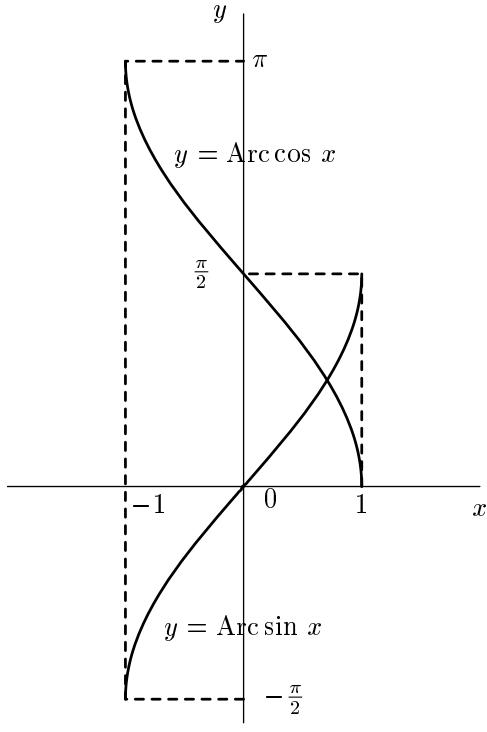
\includegraphics[keepaspectratio]{images/part001_f987f09f.jpg}}\\
Fig. 6

\[
\sin \left(\frac {\pi}{2} - \operatorname{Arc} \cos x\right) = \cos (\operatorname{Arc} \cos x) = x
\]

and since \(-\pi / 2 \leqslant \pi / 2 - \operatorname{Arc} \cos x \leqslant \pi / 2\) , we have

\[
\operatorname{Arc} \cos x = \frac {\pi}{2} - \operatorname{Arc} \sin x\tag{17}
\]

from which in particular it follows that

\[
\mathrm{D} \big (\operatorname{Arc} \cos x \big) = - \frac {1}{\sqrt {1 - x ^ {2}}}.\tag{18}
\]

Finally, the restriction of \(\tan x\) to the interval \(]-\pi/2, +\pi/2[\) is strictly increasing; one denotes its inverse by Arc \(\tan x\) , and this is a strictly increasing map from R onto \(]-\pi/2, +\pi/2[\) (fig.~7); we have

\[
\lim _ {x \rightarrow - \infty} \operatorname{Arc} \tan x = - \frac {\pi}{2}, \quad \lim _ {x \rightarrow + \infty} \operatorname{Arc} \tan x = \frac {\pi}{2},
\]

and, by applying the formula for differentiating inverse functions and formula (15) of III, p.~95, we have

\[
\mathrm{D} \big (\operatorname{Arc} \tan x \big) = \frac {1}{1 + x ^ {2}}.\tag{19}
\]

\pandocbounded{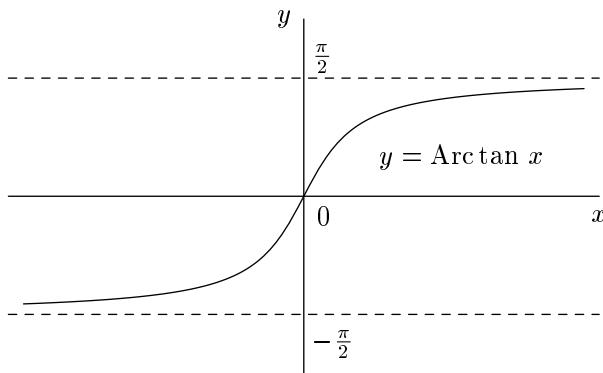
\includegraphics[keepaspectratio]{images/part001_f81b3ea6.jpg}}\\
Fig. 7

\subsection{THE COMPLEX EXPONENTIAL}

We have determined (Gen.~Top., VIII, p.~106) all the continuous homomorphisms of the (additive) topological group C of complex numbers onto the (multiplicative) topological group \(C^{*}\) of complex numbers \(\neq 0\) ; these are the maps

\[
x + i y \mapsto e ^ {\alpha x + \beta y} \mathbf {e} (\gamma x + \delta y)\tag{20}
\]

where \(\alpha, \beta, \gamma, \delta\) are four real numbers subject to the single condition \(\alpha\delta - \beta\gamma \neq 0\) . We now propose to determine which of these homomorphisms \(z \mapsto f(z)\) are differentiable on C. First we remark that it is enough for f to be differentiable at the point z = 0; indeed, for every point \(z \in C\) one has \(\frac{f(z + h) - f(z)}{h} = f(z) \frac{f(h) - 1}{h}\) ; if \(f'(0)\) exists, then so does \(f'(z)\) , and \(f'(z) = af(z)\) , with \(a = f'(0)\) . On the other hand, if g is a second differentiable homomorphism, such that \(g'(z) = bg(z)\) , then \(g(az/b) = f(z)\) , for one notes immediately that the quotient \(g(az/b)/f(z)\) has an everywhere zero derivative and is equal to 1 for z = 0; all the differentiable homomorphisms are thus of the form \(z \mapsto f(\lambda z)\) , where f is one of them (assuming they exist) and \(\lambda\) is any (complex) constant.

This being so, if \(f\) is differentiable at the point \(z = 0\) then each of the maps \(x \mapsto f(x)\) , \(y \mapsto f(iy)\) of \(\mathbf{R}\) into \(\mathbf{C}\) is necessarily differentiable at the point 0, the first having derivative \(f'(0)\) , the second \(if'(0)\) . Now the derivatives of the maps \(x \mapsto e^{\alpha x}\mathbf{e}(\gamma x)\) , \(y \mapsto e^{\beta y}\mathbf{e}(\delta y)\) at the point 0 are respectively equal to \(\alpha + 2\pi i\gamma\) and \(\beta + 2\pi i\delta\) , from which \(\beta = -2\pi\gamma\) and \(\alpha = 2\pi\delta\) ; these conditions are, in particular, satisfied by the homomorphism \(x + iy \mapsto e^x\mathbf{e}(y/2\pi)\) , which we shall denote provisionally by \(f_0\) . We shall now show that \(f_0\) is actually differentiable at the point \(z = 0\) .

It is clear that \(x \mapsto f_0(x)\) and \(y \mapsto f_0(iy)\) have derivatives of every order; in particular, Taylor's formula of order 1 applied to these functions shows that for every \(\varepsilon > 0\) there is an \(r > 0\) such that, if one puts

\[
f _ {0} (x) = 1 + x + \varphi (x) x, \quad f _ {0} (i y) = 1 + i y + \psi (y) y,
\]

then the conditions \(|x| \leqslant r, |y| \leqslant r\) imply that \(|\varphi(x)| \leqslant \varepsilon\) and \(|\psi(y)| \leqslant \varepsilon\) ; this being so, we have \(f_0(x + iy) = f_0(x)f_0(iy) = 1 + (x + iy) + \theta(x, y)\) with

\[
\theta (x, y) = \bigl (i + \varphi (x) \psi (y) \bigr) x y + (1 + x) y \psi (y) + (1 + i y) x \varphi (x);
\]

for \(|z| \leqslant r\) we have \(|x| \leqslant r\) and \(|y| \leqslant r\) , whence

\[
\left| \theta (x, y) \right| \leqslant \left(1 + \varepsilon^ {2}\right) | z | ^ {2} + 2 \varepsilon | z | (1 + | z |)
\]

which proves that the quotient \(\frac{f_{0}(z)-1-z}{z}\) tends to 0 with z, that is to say, the function \(f_{0}\) admits a derivative equal to 1 at the point z=0. The above thus proves that, for all \(z\in C\) ,

\[
\mathrm{D} \big (f _ {0} (z) \big) = f _ {0} (z).\tag{21}
\]

This property establishes the connection between \(f_{0}\) and the function \(e^{x}\) , which is moreover the restriction of \(f_{0}\) to the real axis; for this reason we make the following definition:

DEFINITION 2. The homomorphism \(x + iy \mapsto e^x\mathbf{e}(y/2\pi)\) of \(\mathbf{C}\) onto \(\mathbf{C}^*\) is called the complex exponential; its value at an arbitrary complex number \(z\) is denoted by \(e^z\) or \(\exp z\) .

\subsection{\texorpdfstring{PROPERTIES OF THE FUNCTION \(e^{z}\)}{PROPERTIES OF THE FUNCTION E TO THE Z}}

The fact that \(z \mapsto e^z\) is a homomorphism of \(\mathbf{C}\) onto \(\mathbf{C}^*\) may be expressed by the identities

\[
e ^ {z + z ^ {\prime}} = e ^ {z} e ^ {z ^ {\prime}}, \qquad e ^ {0} = 1, \qquad e ^ {- z} = 1 / e ^ {z}.\tag{22}
\]

By definition, one has, for every \(z = x + iy\) ,

\[
e ^ {x + i y} = e ^ {x} (\cos y + i \sin y)\tag{23}
\]

and since \(e^x > 0\) one sees that \(e^z\) has absolute value \(e^x\) and amplitude \(y\) (modulo \(2\pi\) ).

In particular, def. 2 (III, p.~98) gives

\[
\mathbf {e} (x) = e ^ {2 \pi i x}\tag{24}
\]

which permits us to write the formulae defining \(\cos x\) and \(\sin x\) in the form

\[
\cos x = \frac {1}{2} \left(e ^ {i x} + e ^ {- i x}\right), \quad \sin x = \frac {1}{2 i} \left(e ^ {i x} - e ^ {- i x}\right)\tag{25}
\]

(Euler's formulae).

Since \(2\pi\) is the principal period of \(\mathbf{e}(y/2\pi)\) , \(2\pi i\) is the principal period of \(e^{z}\) ; in other words, the group of periods of \(e^{z}\) is the set of numbers \(2n\pi i\) , where n runs through Z.

Finally, formula (21) of III, p.~98 can be written

\[
\mathrm{D} \left(e ^ {z}\right) = e ^ {z}\tag{26}
\]

whence, for every complex number \(a\)

\[
\mathrm{D} \big (e ^ {a z} \big) = a e ^ {a z}.\tag{27}
\]

Remark. If, in formula (27), one restricts the function \(e^{az}\) (a complex) to the real axis, one again obtains, for x real,

\[
\mathrm{D} (e ^ {a x}) = a e ^ {a x}.\tag{28}
\]

This formula allows us to calculate a primitive for each of the functions \(e^{\alpha x} \cos \beta x\) , \(e^{\alpha x} \sin \beta x\) ( \(\alpha\) and \(\beta\) real); indeed we have \(e^{(\alpha + i\beta)x} = e^{\alpha x} \cos \beta x + ie^{\alpha x} \sin \beta x\) , so, by (28)

\[
\begin{array}{l} \mathrm{D} \left(\mathcal {R} \left(\frac {1}{\alpha + i \beta} e ^ {(\alpha + i \beta) x}\right)\right) = e ^ {\alpha x} \cos \beta x \\ \mathrm{D} \left(\mathcal {I} \left(\frac {1}{\alpha + i \beta} e ^ {(\alpha + i \beta) x}\right)\right) = e ^ {\alpha x} \sin \beta x. \end{array}
\]

In the same way one reduces the evaluation of a primitive of \(x^n e^{\alpha x} \cos \beta x\) , or of \(x^n e^{\alpha x} \sin \beta x\) ( \(n\) an integer \(> 0\) ) to that of a primitive of \(x^n e^{(\alpha + i\beta)x}\) ; now, the formula for integration by parts of order \(n + 1\) (II, p.~60, formula (11)) shows that a primitive of this last function is

\[
e ^ {(\alpha + i \beta) x} \left[ \frac {x ^ {n}}{\alpha + i \beta} - \frac {n x ^ {n - 1}}{(\alpha + i \beta) ^ {2}} + \frac {n (n - 1) x ^ {n - 2}}{(\alpha + i \beta) ^ {3}} + \dots + (- 1) ^ {n} \frac {n !}{(\alpha + i \beta) ^ {n + 1}} \right].
\]

By Euler's formulae one can on the other hand express every positive integral power of \(\cos x\) or of \(\sin x\) as a linear combination of exponentials \(e^{ipx}\) ( \(p\) a positive or negative integer). By formula (28) one can thus express a primitive of a function of the form \(x^n e^{\alpha x}(\cos \beta x)^r (\sin \gamma x)^s\) as a linear combination of functions of the form \(x^p e^{\alpha x}\cos \lambda x\) and \(x^p e^{\alpha x}\sin \mu x\) and \((n, p, r, s\) integers, \(\alpha, \beta, \gamma, \lambda, \mu\) real).

Example. One has

\[
\sin^ {2 n} x = \frac {(- 1) ^ {n}}{2 ^ {2 n}} \left(e ^ {i x} - e ^ {- i x}\right) ^ {2 n} = \frac {(- 1) ^ {n}}{2 ^ {2 n}} \left(e ^ {2 n i x} - \binom {2 n} {1} e ^ {(2 n - 2) i x} + \dots + e ^ {- 2 n i x}\right)
\]

whence

\[
\begin{array}{l} \int_ {0} ^ {x} \sin^ {2 n} t d t = \frac {(- 1) ^ {n}}{2 ^ {2 n}} \left(\frac {1}{n} \sin 2 n x - \binom {2 n} {1} \frac {1}{n - 1} \sin (2 n - 2) x + \dots \right. \\ \qquad \qquad \qquad \qquad \qquad \qquad \qquad \qquad \qquad \qquad + (- 1) ^ {n - 1} \binom {2 n} {n - 1} \sin 2 x + (- 1) ^ {n} \binom {2 n} {n} x \Bigg) \end{array}
\]

and in particular

\[
\int_ {0} ^ {\pi / 2} \sin^ {2 n} t   d t = \binom {2 n} {n} \frac {1}{2 ^ {2 n}}   \frac {\pi}{2} = \frac {1 . 3 . 5 \ldots (2 n - 1)}{2 . 4 . 6 \ldots 2 n}   \frac {\pi}{2}.\tag{29}
\]

\subsection{THE COMPLEX LOGARITHM}

Let B be the ``strip'' formed by the points \(z = x + iy\) such that \(-\pi \leqslant y < \pi\) ; the function \(e^{z}\) takes each of its values once and only once on B; in other words, \(z \mapsto e^{z}\) is a bijective continuous map of B onto \(C^{*}\) ; the image under this map of the (half-open) segment \(x = x_{0}\) , \(-\pi \leqslant y < \pi\) is the circle \(|z| = e^{x_{0}}\) ; the image of the line \(y = y_{0}\) is the (open) half-line defined by \(\operatorname{Am}(z) = y_{0} \pmod{2\pi}\) . The image under \(z \mapsto e^{z}\) of the interior B of B, that is, of the set of \(z \in C\) such that \(|\mathcal{I}(z)| < \pi\) , is the complement F of the (closed) negative real half-axis in C; if one agrees to denote by \(\operatorname{Am}(z)\) the measure of the amplitude of z which belongs to \([-\pi, \pi]\) , then the set F can be defined by the relations \(-\pi < \operatorname{Am}(z) < \pi\) . Since \(z \mapsto e^{z}\) is a strict homomorphism of C onto \(C^{*}\) the image under this map of any open subset of B (so of C) is an open set in \(C^{*}\) (so in F); in other words, the restriction of \(z \mapsto e^{z}\) to B is a homeomorphism of B onto F. We denote by \(z \mapsto \log z\) the homeomorphism of F onto B which is the inverse of the latter; for a complex number \(z \in F\) , \(\log z\) is called the principal value of the logarithm of z. If \(z = x + iy\) and \(\log z = u + iv\) then \(x + iy = e^{u + iv}\) , whence \(e^{u} = |z|\) , and since \(-\pi < v < \pi\) , we have \(v = \operatorname{Am}(z)\) . Moreover, we have \(\tan(v + \pi/2) = -x/y\) if \(y \neq 0\) ; thus we can write

\[
\left\{ \begin{array}{l l} u = \log | z | = \frac {1}{2} \log (x ^ {2} + y ^ {2}) \\ v = \frac {\pi}{2} - \operatorname{Arc} \tan \frac {x}{y} & \text { if } y > 0 \\ v = 0 & \text { if } y = 0 \\ v = - \frac {\pi}{2} - \operatorname{Arc} \tan \frac {x}{y} & \text { if } y <   0. \end{array} \right.\tag{30}
\]

It is clear that \(\log z\) is the extension to F of the function \(\log x\) defined on the positive open real half-axis \(R_{+}^{*}\) . If z, \(z'\) are two points of F such that \(zz'\) is not real negative, we have \(\log(zz') = \log z + \log z' + 2\varepsilon\pi i\) , where \(\varepsilon = +1\) , -1 or 0 depending on the values of \(\mathrm{Am}(z)\) and \(\mathrm{Am}(z')\) .

We note that at the points of the negative real half-axis the function \(\log z\) has no limit; to be precise, if x tends to \(x_{0} < 0\) and if y tends to 0 remaining \textgreater{} 0 (resp. \textless{} 0), then \(\log z\) tends to \(\log |x_{0}| + \pi i\) (resp. \(\log |x_{0}| - \pi i\) ); when z tends to 0, \(|\log z|\) increases indefinitely.

We shall see later how the theory of analytic functions allows us to extend the function \(\log z\) , and to define the complex logarithm in full generality.

Since \(\log z\) is the inverse homeomorphism of \(e^{z}\) , the formula for differentiating inverse functions (I, p.~9, prop. 6) shows that \(\log z\) is differentiable at every point \(z \in F\) , and that

\[
\mathrm{D} (\log z) = \frac {1}{e ^ {\log z}} = \frac {1}{z}\tag{31}
\]

a formula which generalizes formula (10) of III, p.~93.

\subsection{PRIMITIVES OF RATIONAL FUNCTIONS}

Formula (31) allows us to evaluate the primitive of an arbitrary rational function \(r(x)\) of a real variable x, with real or complex coefficients. We know (A.VII.7) that such a function can be written (in unique manner) as a finite sum of terms, which are:

\begin{enumerate}
\def\labelenumi{\alph{enumi})}
\item
  either of the form \(ax^{p}\) (p an integer \(\geqslant 0\) , a a complex number);
\item
  or of the form \(a/(x - b)^{m}\) (m an integer \(\geqslant 0\) , a and b complex numbers).
\end{enumerate}

Now it is easy to obtain a primitive of each of these terms:

\begin{enumerate}
\def\labelenumi{\alph{enumi})}
\tightlist
\item
  a primitive of \(ax^p\) is \(a\frac{x^{p + 1}}{p + 1}\) ;
\end{enumerate}

\(b)\) if \(m > 1\) a primitive of \(a / (x - b)^{m}\) is \(\frac{a}{(1 - m)(x - b)^{m - 1}}\) ;

\begin{enumerate}
\def\labelenumi{\alph{enumi})}
\setcounter{enumi}{2}
\tightlist
\item
  finally, from formulae (10) (III, p.~93) and (31) (III, p.~101), a primitive of \(\frac{a}{x - b}\) is \(a\log |x - b|\) if \(b\) is real, \(a\log (x - b)\) if \(b\) is complex. In the last case, if \(b = p + iq\) , one has furthermore (III, p.~100, formulae (30))
\end{enumerate}

\[
\log (x - b) = \log \sqrt {(x - p) ^ {2} + q ^ {q}} + i \operatorname{Arc} \tan \frac {x - p}{q} \pm i \frac {\pi}{2}.
\]

We postpone the examination of more practical methods for explicitly determining a primitive of a rational function given explicitly to the part of this work dedicated to Numerical Calculus.

One can reduce to the evaluation of a primitive of a rational function:

\(1^{\circ}\) the evaluation of a primitive of a function of the form \(r(e^{ax})\) , where \(r\) is a rational function and \(a\) a real number; indeed by the change of variable \(u = e^{ax}\) one reduces to finding a primitive for \(r(u) / u\) ;

\(2^{\circ}\) the evaluation of a primitive of a function of the form \(f(\sin ax, \cos ax)\) , where \(f\) is a rational function of two variables and \(a\) is a real number; the change of variables \(u = \tan(ax/2)\) reduces this to finding a primitive for

\[
{\frac {2}{1 + u ^ {2}}} f \left({\frac {2 u}{1 + u ^ {2}}}, {\frac {1 - u ^ {2}}{1 + u ^ {2}}}\right).
\]

\subsection{COMPLEX CIRCULAR FUNCTIONS; HYPERBOLIC FUNCTIONS}

Euler's formulae (25) (III, p.~99) and the definition of \(e^z\) for every complex \(z\) allow us to extend to \(\mathbf{C}\) the functions \(\cos x\) and \(\sin x\) defined on \(\mathbf{R}\) , by putting, for all \(z \in \mathbf{C}\)

\[
\cos z = \frac {1}{2} \left(e ^ {i z} + e ^ {- i z}\right), \quad \sin z = \frac {1}{2 i} \left(e ^ {i z} - e ^ {- i z}\right)\tag{32}
\]

(cf.~III, p.~119, exerc. 19).

These functions are periodic with principal period \(2\pi\) ; that is, one has \(\cos(z + \pi/2) = -\sin z\) , \(\sin(z + \pi/2) = \cos z\) ; one may also verify the identities

\[
\begin{array}{c} \cos^ {2} z + \sin^ {2} z = 1 \\ \cos (z + z ^ {\prime}) = \cos z \cos z ^ {\prime} - \sin z \sin z ^ {\prime} \\ \sin (z + z ^ {\prime}) = \sin z \cos z ^ {\prime} + \cos z \sin z ^ {\prime}. \end{array}
\]

More generally, every algebraic identity between circular functions for real variables remains true when one gives these variables arbitrary complex values (III, p.~119, exerc. 18).

One puts \(\tan z = \sin z/\cos z\) if \(z \neq (2k + 1)\pi/2\) and \(\cot z = \cos z/\sin z\) if \(z \neq k\pi\) ; these are periodic functions with principal period \(\pi\) .

Formula (27) (III, p.~99) shows that \(\cos z\) and \(\sin z\) are differentiable on \(\mathbf{C}\) , and that

\[
\mathrm{D} (\cos z) = - \sin z, \quad \mathrm{D} (\sin z) = \cos z.
\]

For \(z = ix\) (x real), the formulae (32) give

\[
\cos i x = \frac {1}{2} \left(e ^ {x} + e ^ {- x}\right), \quad \sin i x = \frac {i}{2} \left(e ^ {x} - e ^ {- x}\right).
\]

It is convenient to have a specific notation for the real functions thus introduced; we put

\[
\left\{ \begin{array}{l l} \cosh x = \frac {1}{2} \left(e ^ {x} + e ^ {- x}\right) & \text {(hyperbolic cosine of x)} \\ \sinh x = \frac {i}{2} \left(e ^ {x} - e ^ {- x}\right) & \text {(hyperbolic sine of x)} \\ \tanh x = \frac {\sinh x}{\cosh x} = \frac {e ^ {x} - e ^ {- x}}{e ^ {x} + e ^ {- x}} & \text {(hyperbolic tangent of x)} \end{array} \right.\tag{33}
\]

One thus has, for every real \(x\)

\[
\cos i x = \cosh x, \quad \sin i x = i \sinh x.\tag{34}
\]

From every identity between circular functions in a certain number of complex numbers \(z_{k}\) ( \(1 \leqslant k \leqslant n\) ) one can deduce an identity for the hyperbolic functions, by replacing \(z_{k}\) by \(ix_{k}\) ( \(x_{k}\) real, \(1 \leqslant k \leqslant n\) ) and using the formulae (34); for instance one has

\[
\begin{array}{c} \cosh^ {2} x - \sinh^ {2} x = 1 \\ \cosh (x + x ^ {\prime}) = \cosh x \cosh x ^ {\prime} + \sinh x \sinh x ^ {\prime} \\ \sinh (x + x ^ {\prime}) = \sinh x \cosh x ^ {\prime} - \cosh x \sinh x ^ {\prime}. \end{array}
\]

The hyperbolic functions allow us to express the real and imaginary parts of \(\cos z\) and \(\sin z\) for \(z = x + iy\) , since

\[
\begin{array}{l} \cos (x + i y) = \cos x \cos i y - \sin x \sin i y = \cos x \cosh y - i \sin x \sinh y \\ \sin (x + i y) = \sin x \cos i y + \cos x \sin i y = \sin x \cosh y + i \cos x \sinh y. \end{array}
\]

Finally, one has

\[
\mathrm{D} (\cosh x) = \sinh x, \mathrm{D} (\sinh x) = \cosh x, \mathrm{D} (\tanh x) = 1 - \tanh ^ {2} x = \frac {1}{\cosh^ {2} x}.
\]

Since \(\cosh x > 0\) for all x one deduces that \(\sinh x\) is strictly increasing on R; since \(\sinh 0 = 0\) , it follows that \(\sinh x\) has the same sign as x. In consequence \(\cosh x\) is strictly decreasing for \(x \leqslant 0\) , strictly increasing for \(x \geqslant 0\) ; finally, \(\tanh x\) is strictly increasing on R. Moreover

\[
\begin{array}{l} \lim _ {x \to - \infty} \sinh x = - \infty , \quad \lim _ {x \to + \infty} \sinh x = + \infty \\ \lim _ {x \to - \infty} \cosh x = \lim _ {x \to + \infty} \cosh x = + \infty \\ \lim _ {x \to - \infty} \tanh x = - 1, \quad \lim _ {x \to + \infty} \tanh x = + 1 \quad (\text {   fig.   8   and   9   }). \end{array}
\]

Sometimes we write \(\operatorname{Arg}\sinh x\) for the inverse function of \(\sinh x\) , which is a strictly increasing map from \(\mathbf{R}\) onto \(\mathbf{R}\) ; this function can also be expressed in terms of the logarithm, since from the relation \(x = \sinh y = \frac{1}{2}(e^y - e^{-y})\) we deduce that \(e^{2y} - 2xe^y - 1 = 0\) , and since \(e^y > 0\) , we have \(e^y = x + \sqrt{x^2 + 1}\) , that is to say

\[
\operatorname{Arg} \sinh x = \log (x + \sqrt {x ^ {2} + 1}).
\]

Similarly, we denote by \(\operatorname{Arg}\cosh x\) the inverse of the restriction of \(\cosh x\) to \([0, +\infty[\) ; this map is strictly increasing from \([1, +\infty[\) onto \([0, +\infty[\) ; one shows as above that

\[
\operatorname{Arg} \cosh x = \log (x + \sqrt {x ^ {2} - 1}).
\]

\pandocbounded{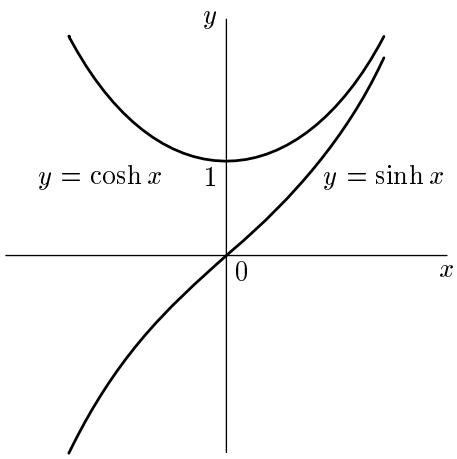
\includegraphics[keepaspectratio]{images/part001_d9e35212.jpg}}\\
Fig. 8

\pandocbounded{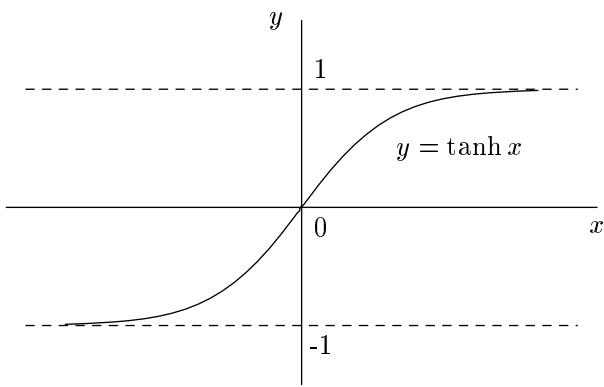
\includegraphics[keepaspectratio]{images/part001_f5896466.jpg}}\\
Fig. 9

Finally, we denote by \(\operatorname{Arg}\tanh x\) the inverse function of \(\tanh x\) , which is a strictly increasing map from \(] - 1, +1[\) onto \(\mathbf{R}\) ; one has, moreover,

\[
\operatorname{Arg} \tanh x = \frac {1}{2} \log \frac {1 + x}{1 - x}.
\]

Remark. For complex \(z\) one sometimes writes

\[
\begin{array}{l} \cosh z = \frac {1}{2} (e ^ {z} + e ^ {- z}) = \cos i z \\ \sinh z = \frac {1}{2} (e ^ {z} - e ^ {- z}) = - i \sin i z. \end{array}
\]

These functions thus extend to C the hyperbolic functions defined on R.

\section{EXPANSIONS OF THE EXPONENTIAL AND CIRCULAR FUNCTIONS, AND OF THE FUNCTIONS ASSOCIATED WITH THEM}

\subsection{EXPANSION OF THE REAL EXPONENTIAL}

Since \(\mathrm{D}^n (e^x) = e^x\) the Taylor expansion of order \(n\) for \(e^x\) is

\[
e ^ {x} = 1 + \frac {x}{1 !} + \frac {x ^ {2}}{2 !} + \dots + \frac {x ^ {n}}{n !} + \int_ {0} ^ {x} \frac {(x - t) ^ {n}}{n !} e ^ {t} d t.\tag{1}
\]

The remainder in this formula is \(>0\) for \(x > 0\) and has the sign of \((-1)^{n + 1}\) when \(x < 0\) ; moreover, the inequality of the mean shows that

\[
\frac {x ^ {n + 1}}{(n + 1) !} <   \int_ {0} ^ {x} \frac {(x - t) ^ {n}}{n !} e ^ {t} d t <   \frac {x ^ {n + 1} e ^ {x}}{(n + 1) !} \quad \text { for } x > 0\tag{2}
\]

\[
\frac {\left| x ^ {n + 1} \right| e ^ {x}}{(n + 1) !} <   \left| \int_ {0} ^ {x} \frac {(x - t) ^ {n}}{n !} e ^ {t} d t \right| <   \frac {\left| x ^ {n + 1} \right|}{(n + 1) !} \quad \text { for } x <   0\tag{3}
\]

Now one knows that the sequence \((x^{n}/n!)\) has limit 0 when n increases indefinitely, for all \(x \geqslant 0\) (Gen.~Top., IV, p.~365); thus, keeping x fixed and letting n grow indefinitely in (1) it follows, from (2) and (3), that

\[
e ^ {x} = \sum_ {n = 0} ^ {\infty} \frac {x ^ {n}}{n !}\tag{4}
\]

and the series on the right-hand side is absolutely and uniformly convergent on every compact interval in \(\mathbf{R}\) . In particular, one has the formula

\[
e = 1 + \frac {1}{1 !} + \frac {1}{2 !} + \dots + \frac {1}{n !} + \dots\tag{5}
\]

This formula allows us to calculate rational approximations as close as we desire to the number \(e\) ; one obtains

\[
e = 2. 7 1 8   2 8 1   8 2 8 \dots
\]

to within \(1/10^{9}\) . Formula (5) proves, moreover, that e is an irrational number \(^{2}\) (Gen.~Top., IV, p.~375).

Remark. Since the remainder in formula (1) is \textgreater0 for x \textgreater{} 0 one has, for x \textgreater{} 0

\[
e ^ {x} > 1 + \frac {x}{1 !} + \frac {x ^ {2}}{2 !} + \dots + \frac {x ^ {n + 1}}{(n + 1) !}
\]

and a fortiori

\[
e ^ {x} > \frac {x ^ {n + 1}}{(n + 1) !}
\]

for every integer \(n\) : one deduces from this that \(e^x / x^n\) tends to \(+\infty\) with \(x\) , for every integer \(n\) : we shall find this result again in chap.~V by another method (V, p.~231).

\subsection{\texorpdfstring{EXPANSIONS OF THE COMPLEX EXPONENTIAL, OF \(\cos x\) AND \(\sin x\).}{EXPANSIONS OF THE COMPLEX EXPONENTIAL, OF COS X AND SIN X}}

Let z be an arbitrary complex number and consider the function \(\varphi(t) = e^{zt}\) of the real variable t; we have \(\mathrm{D}^{n}\varphi(t) = z^{n}e^{zt}\) and \(e^{z} = \varphi(1)\) ; expressing \(\varphi(1)\) by means of its Taylor series of order n about the point t = 0 (II, p.~62) thus gives

\[
e ^ {z} = 1 + \frac {z}{1 !} + \frac {z ^ {2}}{2 !} + \dots + \frac {z ^ {n}}{n !} + z ^ {n + 1} \int_ {0} ^ {1} \frac {(1 - t) ^ {n}}{n !} e ^ {z t} d t\tag{6}
\]

a formula which is equivalent to (1) when \(z\) is real. The remainder

\[
r _ {n} (z) = z ^ {n + 1} \int_ {0} ^ {1} \frac {(1 - t) ^ {n}}{n !} e ^ {z t} d t
\]

in this formula can be bounded above, in absolute value, by using the inequality of the mean; if \(z = x + iy\) we have \(|e^{zt}| = e^{xt}\) , so \(|e^{zt}| \leqslant 1\) if \(x \leqslant 0\) , \(|e^{zt}| \leqslant e^x\) if \(x > 0\) ; hence

\[
\left| r _ {n} (z) \right| \leqslant \frac {\left| z \right| ^ {n + 1}}{(n + 1) !} \text {   if   } x \leqslant 0\tag{7}
\]

\[
| r _ {n} (z) | \leqslant \frac {| z | ^ {n + 1} e ^ {x}}{(n + 1) !} \text {   if   } x > 0.\tag{8}
\]

As above we conclude that

\[
e ^ {z} = \sum_ {n = 0} ^ {\infty} \frac {z ^ {n}}{n !}\tag{9}
\]

the series being absolutely and uniformly convergent on every compact subset of \(\mathbf{C}\) . From (6) one deduces in particular that

\[
e ^ {i x} = 1 + \frac {i x}{1 !} + \frac {i ^ {2} x ^ {2}}{2 !} + \dots + \frac {i ^ {n} x ^ {n}}{n !} + i ^ {n + 1} \int_ {0} ^ {x} \frac {(x - t) ^ {n}}{n !} e ^ {i t} d t\tag{10}
\]

from which we deduce the Taylor expansions of \(\cos x\) and \(\sin x\) ; on taking the real part of (10) for order \(2n + 1\) we have

\[
\cos x = 1 - \frac {x ^ {2}}{2 !} + \dots + (- 1) ^ {n} \frac {x ^ {2 n}}{(2 n) !} + (- 1) ^ {n + 1} \int_ {0} ^ {x} \frac {(x - t) ^ {2 n + 1}}{(2 n + 1) !} \cos t d t\tag{11}
\]

with remainder bounded by

\[
\left| \int_ {0} ^ {x} \frac {(x - t) ^ {2 n + 1}}{(2 n + 1) !} \cos t d t \right| \leqslant \frac {| x | ^ {2 n + 2}}{(2 n + 2) !}.\tag{12}
\]

Similarly, taking the imaginary part of (10) for order \(2n\) , we obtain

\[
\begin{array}{l} \sin x = x - \frac {x ^ {3}}{3 !} + \frac {x ^ {5}}{5 !} + \dots + (- 1) ^ {n - 1} \frac {x ^ {2 n - 1}}{(2 n - 1) !} \\ \qquad + (- 1) ^ {n} \int_ {0} ^ {x} \frac {(x - t) ^ {2 n}}{(2 n) !} \cos t d t \end{array}\tag{13}
\]

with remainder bounded by

\[
\left| \int_ {0} ^ {x} \frac {(x - t) ^ {2 n}}{(2 n) !} \cos t d t \right| \leqslant \frac {| x | ^ {2 n + 1}}{(2 n + 1) !}.\tag{14}
\]

Moreover, on comparing the remainders in (11) for orders \(2n + 1\) and \(2n + 3\) , we have

\[
\int_ {0} ^ {x} \frac {(x - t) ^ {2 n + 3}}{(2 n + 3) !} \cos t d t = \frac {x ^ {2 n + 2}}{(2 n + 2) !} - \int_ {0} ^ {x} \frac {(x - t) ^ {2 n + 1}}{(2 n + 1) !} \cos t d t
\]

and taking (12) into account we see that the remainder in (11) has the same sign as \((-1)^{n+1}\) no matter what x; in the same way we can show that the remainder in (13) has the same sign as \((-1)^{n}x\) . In particular, for n = 0 and n = 1 in (11), and for n = 1 and n = 2 in (13) we obtain the inequalities

\[
1 - \frac {x ^ {2}}{2} \leqslant \cos x \leqslant 1 \quad \text { for   all } x\tag{15}
\]

\[
x - \frac {x ^ {3}}{6} \leqslant \sin x \leqslant x \quad \text { for   all } x \geqslant 0.\tag{16}
\]

Finally, on putting z = ix in (9) we have

\[
\cos x = \sum_ {n = 0} ^ {\infty} (- 1) ^ {n} \frac {x ^ {2 n}}{(2 n) !}\tag{17}
\]

\[
\sin x = \sum_ {n = 0} ^ {\infty} (- 1) ^ {n} \frac {x ^ {2 n + 1}}{(2 n + 1) !}\tag{18}
\]

these series being absolutely and uniformly convergent on every compact interval.

It is clear, furthermore, that the formulae (17) and (18) remain valid for every complex x, the series on the right-hand side being absolutely and uniformly convergent on every compact subset of C. In particular, for every x (real or complex)

\[
\begin{array}{l} \cosh x = \sum_ {n = 0} ^ {\infty} \frac {x ^ {2 n}}{(2 n) !} \\ \sinh x = \sum_ {n = 0} ^ {\infty} \frac {x ^ {2 n + 1}}{(2 n + 1) !}. \end{array}
\]

\subsection{THE BINOMIAL EXPANSION}

Let \(m\) be an arbitrary real number. For \(x > 0\) we have

\[
\mathrm{D} ^ {n} (x ^ {m}) = m (m - 1) \dots (m - n + 1) x ^ {m - n};
\]

the Taylor formula of order \(n\) about the point \(x = 0\) for the function \((1 + x)^m\) shows that for every \(x > -1\)

\[
(1 + x) ^ {m} = 1 + \binom {m} {1} x + \binom {m} {2} x ^ {2} + \dots + \binom {m} {n} x ^ {n} + r _ {n} (x)\tag{19}
\]

with

\[
r _ {n} (x) = \frac {m (m - 1) \dots (m - n)}{n !} \int_ {0} ^ {x} \left(\frac {x - t}{1 + t}\right) ^ {n} (1 + t) ^ {m - 1} d t
\]

where we put \(\binom{m}{n} = \frac{m(m-1)\ldots(m-n+1)}{n!}\) . The formula (19) reduces to the binomial formula (Alg., I, p.~99) when m is an integer \textgreater{} 0 and \(n \geqslant m\) ; by extension, we again call it the binomial formula, and the coefficients \(\binom{m}{n}\) are called the binomial coefficients, when m is an arbitrary real number and n is an arbitrary integer \textgreater{} 0.

The remainder in (19) has the same sign as \(\binom{m}{n+1}\) if \(x > 0\) , and the sign of \((-1)^{n+1}\binom{m}{n+1}\) if \(-1 < x < 0\) . Since \(\left|\frac{x-t}{1+t}\right| \leqslant |x|\) for \(t > -1\) in the interval with endpoints 0 and \(x\) , we have the following bound for the remainder, for \(m\) and \(n\) arbitrary and \(x > -1\) :

\[
\begin{array}{r l} \left| \frac {m (m - 1) \dots (m - n)}{n !} \int_ {0} ^ {x} \left(\frac {x - t}{1 + t}\right) ^ {n} (1 + t) ^ {m - 1} d t \right| & \\ & \leqslant \left| \binom {m - 1} {n} x ^ {n} ((1 + x) ^ {m} - 1) \right|. \end{array}\tag{20}
\]

If we suppose \(x \geqslant 0\) , and \(n \geqslant m - 1\) , then \((1 + t)^{n - m + 1} \geqslant 1\) on the interval of integration, so

\[
0 \leqslant \int_ {0} ^ {x} \frac {(x - t) ^ {n}}{(1 + t) ^ {n - m + 1}} d t \leqslant \int_ {0} ^ {x} (x - t) ^ {n} d t = \frac {x ^ {n + 1}}{n + 1}
\]

which gives the estimate

\[
\left| r _ {n} (x) \right| \leqslant \left| \binom {m} {n + 1} \right| x ^ {n + 1} \quad (x \geqslant 0, n \geqslant m - 1)\tag{21}
\]

for the remainder. On the other hand, suppose that \(-1 \leqslant m < 0\) ; if one makes the change of variable \(u = \frac{x - t}{x(1 + t)}\) in the integral (19) one obtains

\[
r _ {n} (x) = \frac {m (m - 1) \dots (m - n)}{n !} (1 + x) ^ {m} x ^ {n + 1} \int_ {0} ^ {1} \frac {u ^ {n} d u}{(1 + u x) ^ {m + 1}}.\tag{22}
\]

To estimate the integral for x \textgreater{} -1 we remark that, since \(m + 1 < 1\) , the integral \(\int_{0}^{1}\frac{u^{n}du}{(1-u)^{m+1}}\) converges and bounds the right-hand side of (22) since \(1+ux > 1-u\) . Now, for -1 \textless{} x \textless{} 0 the hypothesis on m implies that all the terms \(\binom{m}{1}x,\binom{m}{2}x^{2},\ldots,\binom{m}{n}x^{n}\) which appear in the right-hand side of (19) are \(\geqslant 0\) , and hence \(r_{n}(x) \leqslant (1+x)^{m}\) , from which, on dividing by \((1+x)^{m}\) ,

\[
\frac {m (m - 1) \dots (m - n)}{n !} x ^ {n + 1} \int_ {0} ^ {1} \frac {u ^ {n} d u}{(1 + u x) ^ {m + 1}} \leqslant 1.
\]

Moreover, for \(-1 < x < 0\) the factor in front of the integral is \(\geqslant 0\) , so, letting \(x\) approach \(-1\) ,

\[
\left| \frac {m (m - 1) \dots (m - n)}{n !} \int_ {0} ^ {1} \frac {u ^ {n} d u}{(1 - u) ^ {m + 1}} \right| \leqslant 1
\]

and consequently for \(-1 \leqslant m < 0\) and \(x > -1\) we have

\[
\left| r _ {n} (x) \right| \leqslant (1 + x) ^ {m} | x | ^ {n + 1}.\tag{23}
\]

From these inequalities we can, for a start, deduce that for \(|x| < 1\) we have

\[
(1 + x) ^ {m} = \sum_ {n = 0} ^ {\infty} \binom {m} {n} x ^ {n}\tag{24}
\]

the right-hand side (called the binomial series) being absolutely and uniformly convergent on every compact subset of {]} - 1, +1{[}. Indeed one can write

\[
\binom {m} {n} = (- 1) ^ {n} \left(1 - \frac {m + 1}{1}\right) \left(1 - \frac {m + 1}{2}\right) \dots \left(1 - \frac {m + 1}{n}\right)\tag{25}
\]

whence

\[
\left| \binom {m} {n} \right| \leqslant \left(1 + \frac {| m + 1 |}{1}\right) \left(1 + \frac {| m + 1 |}{2}\right) \dots \left(1 + \frac {| m + 1 |}{n}\right).
\]

If \(|x| \leqslant r < 1\) there is an \(n_0\) such that \(1 + \frac{|m|}{n_0} < \frac{1}{r'}\) , where \(r < r' < 1\) ; whence, putting

\[
k = \left(1 + \frac {| m |}{1}\right) \left(1 + \frac {| m |}{2}\right) \dots \left(1 + \frac {| m |}{n _ {0}}\right)
\]

we have

\[
\left| \binom {m - 1} {n} x ^ {n} \right| \leqslant k | x | ^ {n _ {0}} \left(\frac {r}{r ^ {\prime}}\right) ^ {n - n _ {0}},
\]

which proves the proposition. On the other hand, for x \textgreater{} 1, the absolute value of the general term of the series (24) increases indefinitely with n if m is not an integer \(\geqslant 0\) ; indeed, from (25), we have for \(n > n_{1} \geqslant |m + 1|\)

\[
\begin{array}{r l} \left| \binom {m} {n} \right| & \geqslant \left| \left(1 - \frac {m + 1}{1}\right) \left(1 - \frac {m + 1}{2}\right) \dots \left(1 - \frac {m + 1}{n _ {1}}\right) \right| \\ & \quad \left(1 - \frac {| m + 1 |}{n _ {1} + 1}\right) \dots \left(1 - \frac {| m + 1 |}{n}\right). \end{array}
\]

Let \(n_0 \geqslant n_1\) be such that for \(n \geqslant n_0\) we have \(1 - \frac{|m + 1|}{n} > \frac{1}{x'}\) , where \(1 < x' < x\) . If we put

\[
k ^ {\prime} = \left| \left(1 - \frac {m + 1}{1}\right) \dots \left(1 - \frac {m + 1}{n _ {1}}\right) \right| \left(1 - \frac {| m + 1 |}{n _ {1} + 1}\right) \dots \left(1 - \frac {| m + 1 |}{n _ {0}}\right)
\]

then, for \(n > n_0\) ,

\[
\left| \binom {m} {n} x ^ {n} \right| \geqslant k ^ {\prime} | x | ^ {n _ {0}} \left(\frac {x}{x ^ {\prime}}\right) ^ {n - n _ {0}}
\]

from which the proposition follows.

We remark that for \(m = -1\) the algebraic identity

\[
\frac {1}{1 + x} = 1 - x + x ^ {2} - \dots + (- 1) ^ {n - 1} x ^ {n - 1} + (- 1) ^ {n} \frac {x ^ {n}}{1 + x}\tag{26}
\]

gives the expression for the remainder in the general formula (19) without having to integrate; the formula (23) reduces in this case to the expression for the sum of the geometric series (or progression) (Gen.~Top., IV, p.~364).

In the second place let us study the convergence of the binomial series for \(x = 1\) or \(x = -1\) (excluding the trivial case \(m = 0\) ):

\begin{enumerate}
\def\labelenumi{\alph{enumi})}
\item
  \(m \leqslant -1\) . The product with general term \(1 - \frac{m + 1}{n}\) converges to \(+\infty\) if \(m < -1\) , to 1 if \(m = -1\) , so it follows from (25) that for \(x = \pm 1\) the general term of the binomial series does not tend to 0.
\item
  -1 \textless{} m \textless{} 0. This time the product with general term \(1 - \frac{m + 1}{n}\) converges to 0, so the inequality (21) shows that \(r_{n}(1)\) tends to 0. Thus the binomial series converges for x = 1 and has sum \(2^{m}\) ; moreover, the binomial series is uniformly convergent on every interval \([x_{0}, 1]\) with \(-1 < x_{0} \leqslant 1\) , by virtue of what we saw above and of (21). On the other hand, for x = -1 all the terms on the right-hand side of (24) are \(\geqslant 0\) ; if this series were convergent one could deduce that the binomial series would be normally convergent on \([-1, 1]\) and so would have for its sum a continuous function on this interval, which is absurd because \((1 + x)^{m}\) is not bounded on \([-1, 1]\) for m \textless{} 0. We conclude that also for x = 1 the binomial series is not absolutely convergent.
\item
  m \textgreater{} 0. The definition of \(r_{n}(x)\) shows that \(r_{n}(x)\) tends to the limit \(r_{n}(-1)\) when x tends to -1; on passing to the limit in (20) one concludes that \(|r_{n}(-1)| \leqslant \left|\binom{m-1}{n}\right|\) , and since m - 1 \textgreater{} -1 we see that for x = -1 the binomial series is convergent. Furthermore, for \(n > m + 1\) all the terms of this series have the same sign; thus the binomial series is normally convergent on the interval \([-1, 1]\) and has sum \((1 + x)^{m}\) on this interval.
\end{enumerate}

\subsection{\texorpdfstring{EXPANSIONS OF \(\log(1 + x)\), OF Arc tan x AND OF Arc sin x}{EXPANSIONS OF LOG(1 + X), ARC TAN X AND ARC SIN X}}

Let us integrate the two sides of (26) between 0 and x; we obtain the Taylor expansion of order n of \(\log(1 + x)\) , valid for x \textgreater{} -1

\[
\log (1 + x) = \frac {x}{1} - \frac {x ^ {2}}{2} + \frac {x ^ {3}}{3} + \dots + (- 1) ^ {n - 1} \frac {x ^ {n}}{n} + (- 1) ^ {n} \int_ {0} ^ {x} \frac {t ^ {n} d t}{1 + t}.\tag{27}
\]

The remainder has the same sign as \((-1)^{n}\) if x \textgreater{} 0, and is \textless{} 0 if -1 \textless{} x \textless{} 0; further, when x \textgreater{} 0, we have \(1 + t \geqslant 1\) for \(0 \leqslant t \leqslant x\) , and, when -1 \textless{} x \textless{} 0, we have \(1 + t \geqslant 1 - |x|\) for \(x \leqslant 0\) ; whence the estimates for the remainder

\[
\left| \int_ {0} ^ {x} \frac {t ^ {n} d t}{1 + t} \right| \leqslant \frac {| x | ^ {n + 1}}{n + 1}
\]

\[
\text { for } x \geqslant 0\tag{28}
\]

\[
\left| \int_ {0} ^ {x} \frac {t ^ {n} d t}{1 + t} \right| \leqslant \frac {| x | ^ {n + 1}}{(n + 1) (1 - | x |)} \quad \text {   for   } - 1 <   x \leqslant 0.\tag{29}
\]

From these last two formulae one deduces immediately that for \(-1 < x \leqslant 1\) one has

\[
\log (1 + x) = \sum_ {n = 1} ^ {\infty} (- 1) ^ {n - 1} \frac {x ^ {n}}{n}\tag{30}
\]

the series being uniformly convergent on every compact interval contained in \(]-1,+1]\) , and absolutely convergent for \(|x|<1\) .

On the other hand, for \(|x| > 1\) the general term in the series on the right-hand side of (30) increases indefinitely in size with n (III, p.~106). For x = -1 the series reduces to the harmonic series, which has sum \(+\infty\) (Gen.~Top., IV, p.~365).

Similarly, let us replace \(x\) by \(x^2\) in (26) and integrate both sides between 0 and \(x\) ; we obtain the Taylor expansion of order \(2n - 1\) for \(\operatorname{Arctan} x\) , valid for all real \(x\)

\[
\operatorname{Arc} \tan x = \frac {x}{1} - \frac {x ^ {3}}{3} + \frac {x ^ {5}}{5} + \dots + (- 1) ^ {n - 1} \frac {x ^ {2 n - 1}}{2 n - 1} + (- 1) ^ {n} \int_ {0} ^ {x} \frac {t ^ {2 n} d t}{1 + t ^ {2}}.\tag{31}
\]

The remainder has the sign of \((-1)^n x\) , and since \(1 + t^2 \geqslant 1\) for all \(t\) we have the estimate

\[
\left| \int_ {0} ^ {x} \frac {t ^ {2 n} d t}{1 + t ^ {2}} \right| \leqslant \frac {| x | ^ {2 n + 1}}{2 n + 1}\tag{32}
\]

from which one deduces that, for \(|x| \leqslant 1\) ,

\[
\operatorname{Arc} \tan x = \sum_ {n = 1} ^ {\infty} (- 1) ^ {n - 1} \frac {x ^ {2 n - 1}}{2 n - 1}\tag{33}
\]

the series being uniformly convergent on \([-1,+1]\) , and absolutely convergent for \(|x|<1\) .

In particular, for \(x = 1\) one obtains the formula

\[
{\frac {\pi}{4}} = 1 - {\frac {1}{3}} + {\frac {1}{5}} + \dots + (- 1) ^ {n} {\frac {1}{2 n + 1}} + \dots .\tag{34}
\]

For \(|x| > 1\) the general term of the right-hand side of (33) increases indefinitely in size with \(n\) .

Finally, for the Taylor expansion of Arc sin x we start from the expansion of its derivative \((1 - x^{2})^{-1/2}\) ; this last expansion is obtained by replacing x by \(-x^{2}\) in the expansion of \((1 + x)^{-1/2}\) as a binomial series; for \(|x| < 1\) this gives

\[
(1 - x ^ {2}) ^ {- 1 / 2} = 1 + \frac {1}{2} x ^ {2} + \frac {1 . 3}{2 . 4} x ^ {4} + \dots + \frac {1 . 3 . 5 \dots (2 n - 1)}{2 . 4 . 6 \dots 2 n} x ^ {2 n} + r _ {n} (x)
\]

with, by (23), the bound

\[
0 \leqslant r _ {n} (x) \leqslant \frac {x ^ {2 n + 2}}{\sqrt {1 - x ^ {2}}}
\]

for the remainder.

On taking the primitive of the preceding expansion we obtain

\[
\operatorname{Arc} \sin x = x + \frac {1}{2} \frac {x ^ {3}}{3} + \frac {1 . 3}{2 . 4} \frac {x ^ {5}}{5} + \dots + \frac {1 . 3 . 5 \dots (2 n - 1)}{2 . 4 . 6 \dots 2 n} \frac {x ^ {2 n + 1}}{2 n + 1} + \mathrm{R} _ {n} (x)\tag{35}
\]

where \(\mathrm{R}_{n}(x)\) has the sign of x and satisfies the inequality

\[
| \mathrm{R} _ {n} (x) | \leqslant \int_ {0} ^ {x} \frac {t ^ {2 n + 2} d t}{\sqrt {1 - t ^ {2}}}.\tag{36}
\]

Further, the relation (35) shows that \(\mathbf{R}_n(x)\) tends to a limit when \(x\) approaches 1 or \(-1\) , so one has

\[
| \mathrm{R} _ {n} (1) | \leqslant \int_ {0} ^ {1} \frac {t ^ {2 n + 2} d t}{\sqrt {1 - t ^ {2}}}.\tag{37}
\]

But the right-hand side of (37) tends to 0 when \(n\) tends to \(+\infty\) : for, since the integral \(\int_0^1 dt / \sqrt{1 - t^2}\) is convergent, for every \(\varepsilon > 0\) there is an \(a\) such that \(0 < a < 1\) and \(\int_a^1 dt / \sqrt{1 - t^2} \leqslant \varepsilon\) ; on the other hand we have

\[
\int_ {0} ^ {a} \frac {t ^ {2 n + 2} d t}{\sqrt {1 - t ^ {2}}} \leqslant \frac {1}{\sqrt {1 - a ^ {2}}} \int_ {0} ^ {a} t ^ {2 n + 2} d t = \frac {a ^ {2 n + 3}}{(2 n + 3) \sqrt {1 - a ^ {2}}}
\]

and so there is an \(n_0\) such that for \(n \geqslant n_0\) one has \(\frac{a^{2n+3}}{(2n+3)\sqrt{1-a^2}} \leqslant \varepsilon\) , whence, finally, \(|\mathrm{R}_n(x)| \leqslant 2\varepsilon\) for \(|x| \leqslant 1\) and \(n \geqslant n_0\) . Thus one has

\[
\operatorname{Arc} \sin x = \sum_ {n = 0} ^ {\infty} \frac {1 . 3 . 5 \dots (2 n - 1)}{2 . 4 . 6 \dots 2 n} \frac {x ^ {2 n + 1}}{2 n + 1}\tag{38}
\]

the right-hand side being normally convergent on the compact interval \([-1, 1]\) .

In the opposite case one can show, as for the binomial series, that the general term in the series on the right-hand side of (38) increases indefinitely in absolute value for \(|x| > 1\) .

On putting \(x = \frac{1}{2}\) , for example, in (38) we obtain a new expression for the number \(\pi\) ;

\[
\frac {\pi}{6} = \sum_ {n = 0} ^ {\infty} \frac {1 . 3 . 5 \dots (2 n - 1)}{2 . 4 . 6 \dots 2 n} \frac {1}{(2 n + 1) 2 ^ {2 n + 1}}
\]

which is much better suited than formula (34) to calculating approximations to \(\pi\) (see Calcul numérique); one thus obtains

\[
\pi = 3. 1 4 1   5 9 2   6 5 3 \dots
\]

accurate to within \(1/10^{9}\) . \(^{3}\)
